%%%%%%%%%%%%%%%%%%%%%%%%%%%%%%%%%%%%%%%%%
% Stylish Article
% LaTeX Template
% Version 2.2 (2020-10-22)
%
% This template has been downloaded from:
% http://www.LaTeXTemplates.com
%
% Original author:
% Mathias Legrand (legrand.mathias@gmail.com) 
% With extensive modifications by:
% Vel (vel@latextemplates.com)
%
% License:
% CC BY-NC-SA 3.0 (http://creativecommons.org/licenses/by-nc-sa/3.0/)
%
%%%%%%%%%%%%%%%%%%%%%%%%%%%%%%%%%%%%%%%%%

%----------------------------------------------------------------------------------------
%	PACKAGES AND OTHER DOCUMENT CONFIGURATIONS
%----------------------------------------------------------------------------------------

\documentclass[fleqn,10pt]{SelfArx} % Document font size and equations flushed left

\usepackage[fontset=none]{ctex}
\setCJKmainfont{Noto Serif CJK SC}
\setCJKsansfont{Noto Serif CJK SC}
\setCJKmonofont{Noto Sans CJK SC}

%----------------------------------------------------------------------------------------
%	COLUMNS
%----------------------------------------------------------------------------------------

\setlength{\columnsep}{0.55cm} % Distance between the two columns of text
\setlength{\fboxrule}{0.75pt} % Width of the border around the abstract

%----------------------------------------------------------------------------------------
%	COLORS
%----------------------------------------------------------------------------------------

\definecolor{color1}{RGB}{0,0,90} % Color of the article title and sections
\definecolor{color2}{RGB}{0,20,20} % Color of the boxes behind the abstract and headings

%----------------------------------------------------------------------------------------
%	HYPERLINKS
%----------------------------------------------------------------------------------------

\usepackage{hyperref} % Required for hyperlinks

\hypersetup{
	hidelinks,
	colorlinks,
	breaklinks=true,
	urlcolor=color2,
	citecolor=color1,
	linkcolor=color1,
	bookmarksopen=false,
	pdftitle={Title},
	pdfauthor={Author},
}

%----------------------------------------------------------------------------------------
%	ARTICLE INFORMATION
%----------------------------------------------------------------------------------------

\JournalInfo{基础物理学实验A3} % Journal information
\Archive{} % Additional notes (e.g. copyright, DOI, review/research article)

\PaperTitle{同轴光子晶体实验报告} % Article title

\Authors{} % Authors
\affiliation{} % Author affiliation

\Keywords{} % Keywords - if you don't want any simply remove all the text between the curly brackets
\newcommand{\keywordname}{Keywords} % Defines the keywords heading name

%----------------------------------------------------------------------------------------
%	ABSTRACT
%----------------------------------------------------------------------------------------

\Abstract{本实验利用两种特征阻抗的同轴电缆交替连接构成的特征阻抗周期性变化的结构,形成与能带类似的电磁频带和带隙,模拟了光子晶体的特性。通过理论计算和实验操作,最后在同轴电缆中观察到了类似于光子晶体中的能带结构,折射率特性,超光速与慢光速现象。}

%----------------------------------------------------------------------------------------

\begin{document}

\maketitle % Output the title and abstract box

\tableofcontents % Output the contents section

\thispagestyle{empty} % Removes page numbering from the first page

%----------------------------------------------------------------------------------------
%	ARTICLE CONTENTS
%----------------------------------------------------------------------------------------

\section{理论计算} % The \section*{} command stops section numbering

整个实验我们只用一种型号的$4.8m$长的同轴电缆。先计算同轴电缆的衰减系数$\alpha$。我们通过$V=V_0e^{-\alpha x}$,带入电压减小值,得$\alpha=0.00573$,即输入$1V$的信号,$10m$后为$0.944V$,$20m$后为$0.892V$,$30m$后为$0.842V$。为了引入另一种特征阻抗的同轴电缆,我们使用两段相同的同轴电缆并联,我们可通过推导得到并联电缆的等效性质。由于两根电缆始末段并联相当于电缆的每一种电气性质/结构并联。这样就可求出:$R'=\frac{R'}{2}$,$L'=\frac{L}{2}$,$C'=2C$,$G'=2G$。再计算:$Z_0'=\sqrt{\frac{R'+j\omega L'}{G'+j\omega C'}}=\sqrt{\frac{\frac{1}{2}(R+j\omega L)}{2(G+j\omega C)}}=\frac{Z_0}{2}$。类似的还可算出:$\alpha'=\alpha$,$\beta'=\beta$。根据计算,并联获得了更低的阻抗,而单根电联是高阻抗,即$Z_{OL}=\frac{Z_0}{2}$,$Z_{OH}=Z_0$。故而$Z_{OH}/Z_{OL}=2$。(可看出通过不断并联可以得到更高的阻抗比)最后理论计算第一个通带频率和第一个带隙频率。由通带频率$f_0=\frac{c}{\sqrt{\epsilon_r}\lambda}$,这里$\frac{\lambda}{2}=4.8m$,$\epsilon_r= 2.354$。代入,我们有:通带频率$f_0=20.35MHz$,带隙频率$\frac{f_0}{2}=10.18MHz$。

信号在不同特征阻抗同轴电缆连接处会发生透射与反射。在连接处,两根同轴电缆内外导体间的电压应连续,入射电流应等于反射电流与透射电流之和。推导可得,电压反射系数$\Gamma=\frac{Z_1-Z_0}{Z_1+Z_0}$,电压透射系数$T=\frac{2Z_1}{Z_1+Z_0}$。将前述阻抗关系代入,可知$\Gamma=\frac{1}{3}$,$T=\frac{4}{3}$入射功率$P_i=\frac{V_i^2}{Z_0}$,反射功率$P_r=\frac{V_r^2}{Z_0}=\frac{V_i^2}{9Z_0}$,透射功率$P_t=\frac{V_t^2}{2Z_0}=\frac{8V_i^2}{9Z_0}$,即入射功率等于反射功率与透射功率之和。
%------------------------------------------------

\section{实验操作及数据处理}

我们搭建测试电路,一路直接从信号发生器到示波器(Ch1),一路经过同轴光子晶体(Ch2)。同轴光子晶体由4个低阻(两个同轴并联)和3个高阻交叉串联而成,共$33.6m$。并保证信号发生器两路正弦波的频率,峰值,初相位完全相同。

\paragraph*{无缺陷的情况} 先直接测定$1MHz$到$20MHz$之间的情况,结果如\ref{tab:app1}。我们计算传输效率和等效折射率。传输效率$\eta=P_2/P_1$,这里测定了50欧姆电阻上的电压,由于$P=U^2R$,故两个平方相除即可。等效折射率$n=ct_p/L$,其中$\phi=-\omega t_p$,L为33.6m。最终得到的数据如\ref{tab:app2}。将数据作图,如图\ref{fig:a1}所示。根据图片,我们可以看出,通带在$20MHz$附近,带隙在$10MHz$附近,这与我们的理论计算结果是完全相符的。
\begin{figure}[htbp]
	\centering
	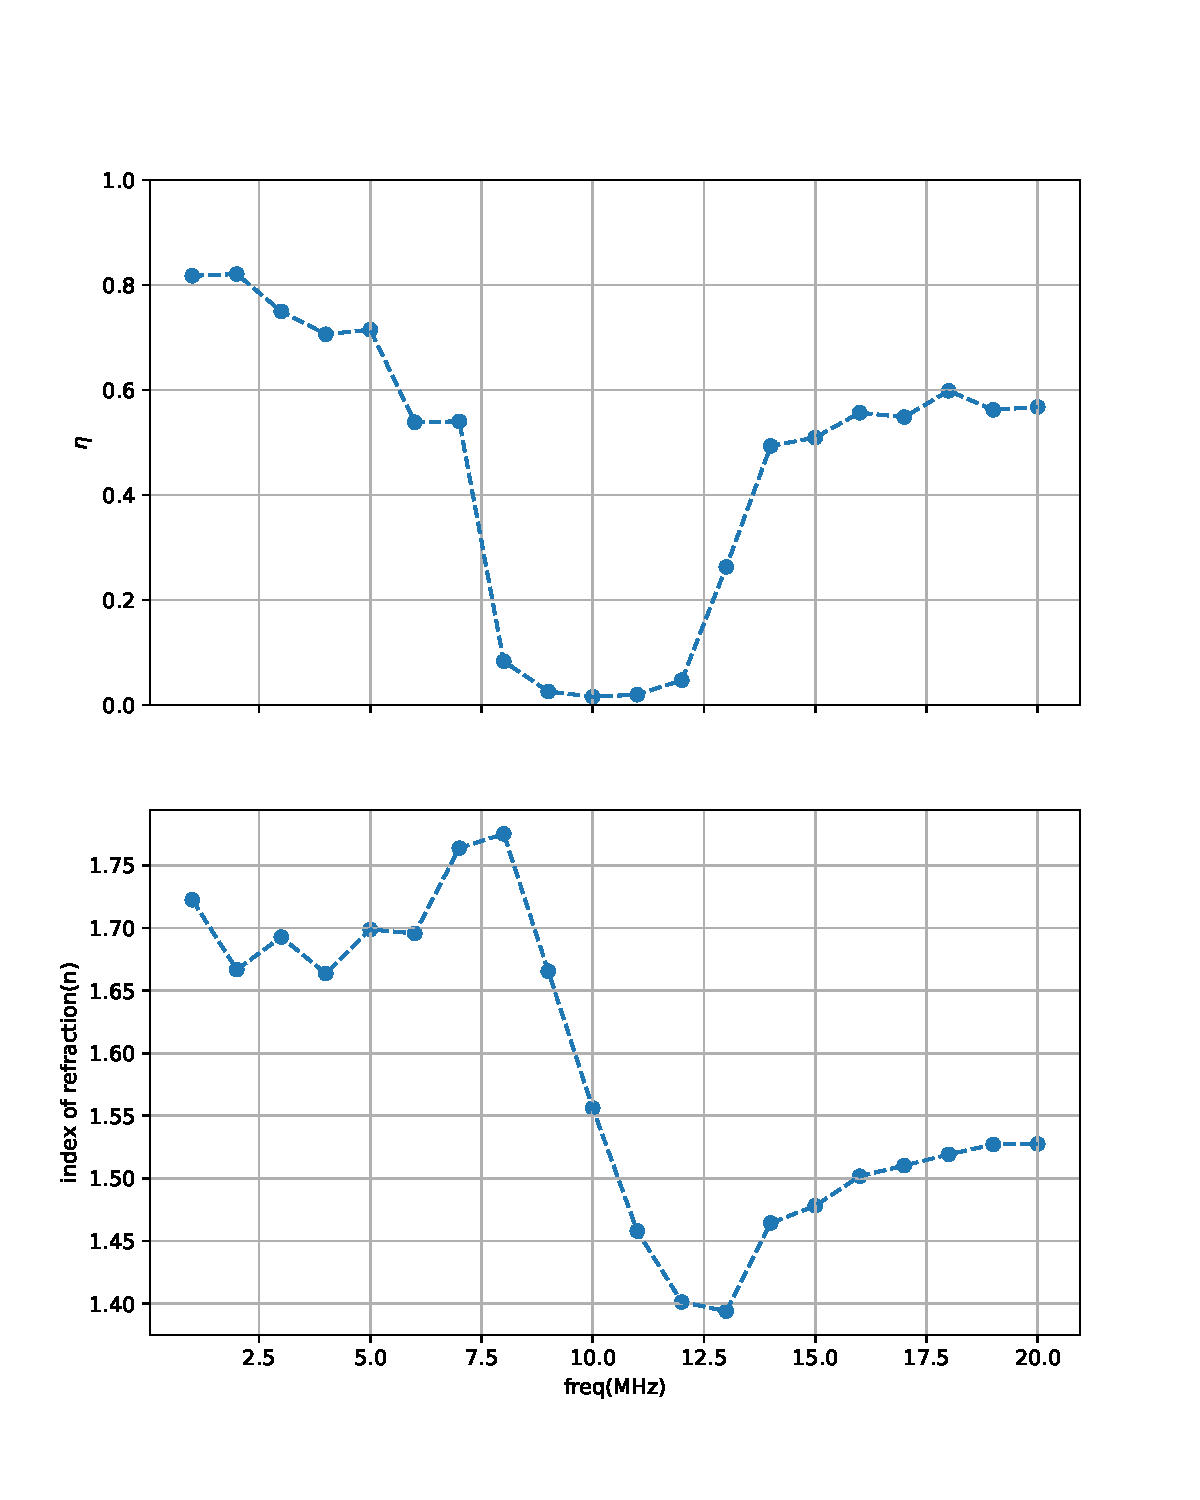
\includegraphics[width=\linewidth]{C1-eta-n.pdf}
	\caption{无缺陷时的传输效率与折射率}
	\label{fig:a1}
\end{figure}

另一个重要的量是群速度,我们计算各个频率处的群速度$v_g=c/(n+\omega\frac{dn}{d\omega})$,结果如\ref{tab:app3}。计算时,我们使用了前后两次之差近似代表微分,故而最终计算出19组数据。画出图,如图\ref{fig:a2}所示。我们再一次在图中看到了带隙,与前面的预测相符。同时,群速度出现了超光速(红线),这并不违反相对论,因为信息传播的速度仍会慢于光速,在后面将看到这一点。
\begin{figure}[htbp]
	\centering
	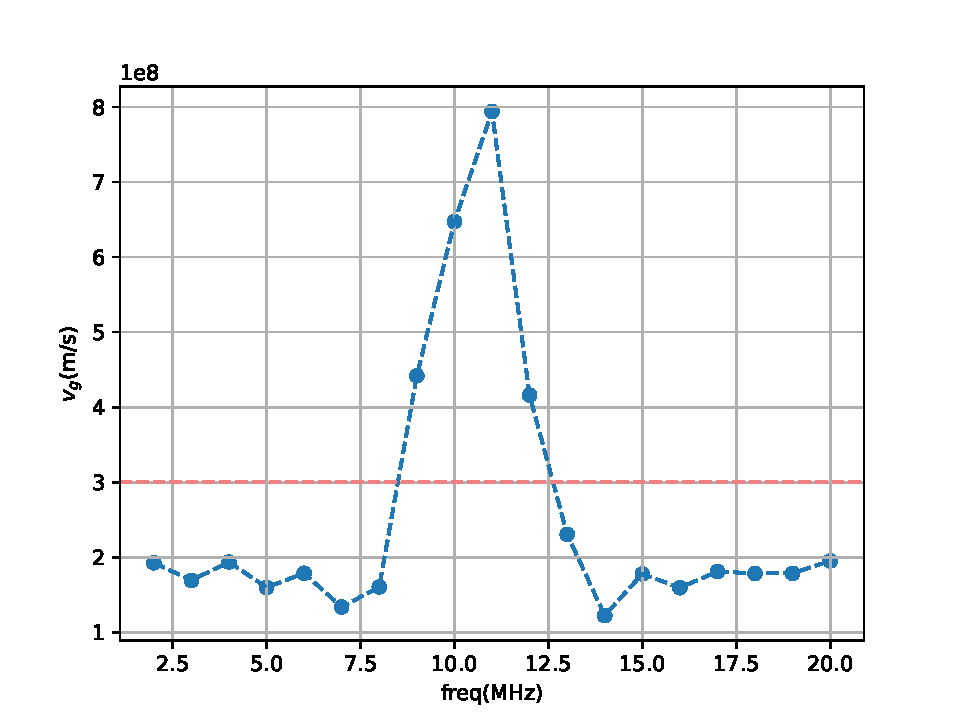
\includegraphics[width=\linewidth]{C1-vg.pdf}
	\caption{无缺陷时的群速度}
	\label{fig:a2}
\end{figure}

\paragraph*{有缺陷的情况} 我们在中间增加一根同轴电缆,破坏对称性,模拟光子晶体的缺陷,此时总长度来到了$38.4m$。与上面相同,测定$1MHz$到$20MHz$之间的情况,结果如\ref{tab:app4}。并计算传输效率和等效折射率,如\ref{tab:app5}。同样,作出图,如图\ref{fig:a3}所示。我们可以看到,在原来的带隙的位置,出现了一个小峰,这就是缺陷破坏对称性的体现。
\begin{figure}[htbp]
	\centering
	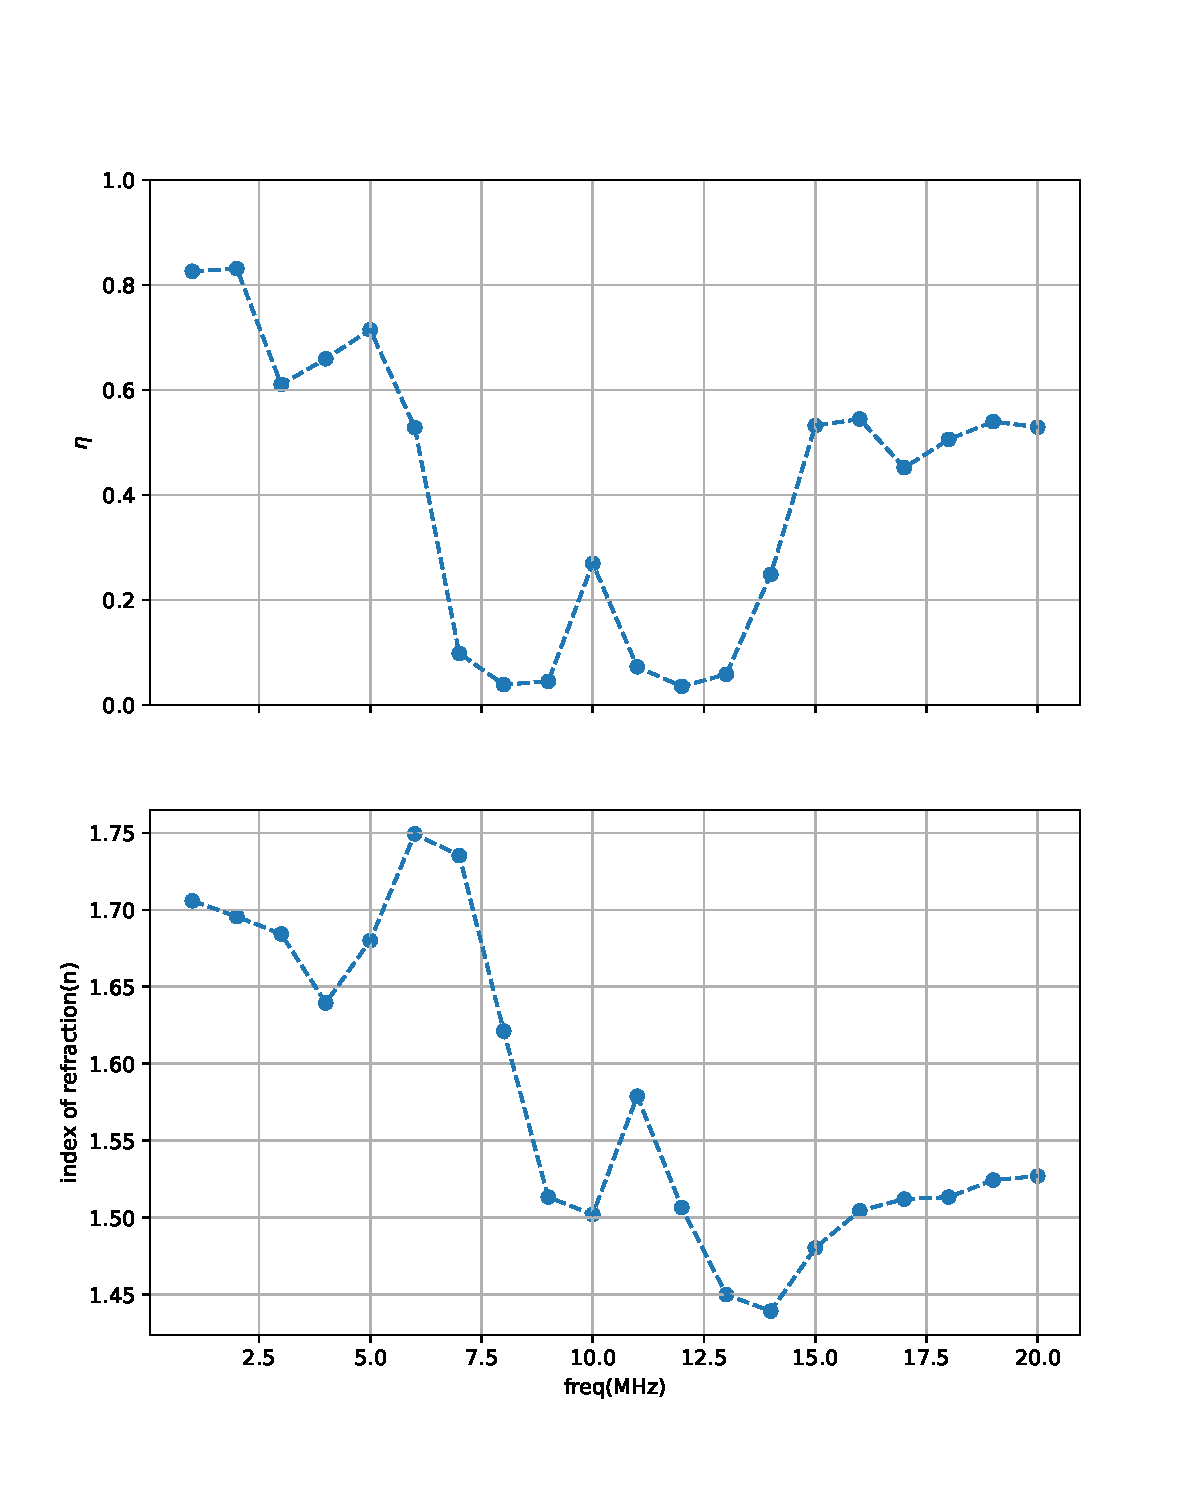
\includegraphics[width=\linewidth]{C4-eta-n.pdf}
	\caption{有缺陷时的传输效率与折射率}
	\label{fig:a3}
\end{figure}

同样,计算群速度,结果如\ref{tab:app6}。作出图,结果如图\ref{fig:a4}所示。同样,我们在原本带隙的位置看到了对称性的破缺,这是在我们意料之中的。
\begin{figure}[htbp]
	\centering
	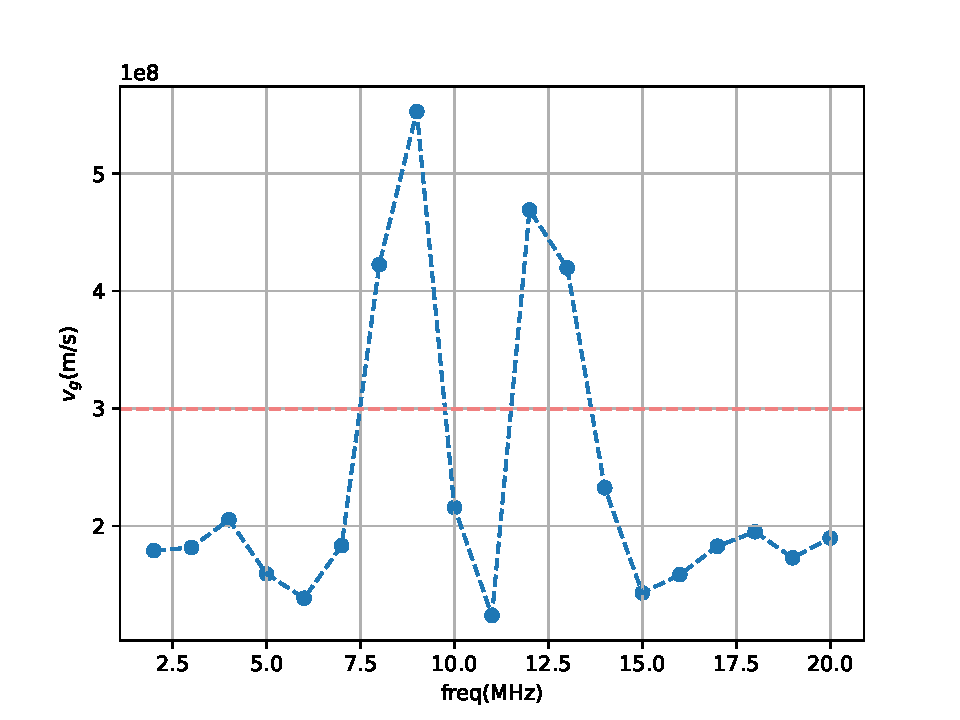
\includegraphics[width=\linewidth]{C4-vg.pdf}
	\caption{有缺陷时的群速度}
	\label{fig:a4}
\end{figure}

\paragraph*{直接测试电磁波脉冲的超光速与慢光速传输现象} 前面我们看到了电磁波的群速度存在超光速的现象,下面我们就详细讨论这一点。同样测定有缺陷时的情况。我们使用一个脉冲信号,在$50kHz$至$150kHz$范围内改变信号发生器频率,找出3个特征频率:信号幅度最小的两个频率、以及这两个频率之间信号幅度最大且延时最长的1个频率。最后还关注$150kHz$,四个频率下的波形如图\ref{fig:a5},\ref{fig:a6},\ref{fig:a7},\ref{fig:a8}所示。
\begin{figure}[htbp]
	\centering
	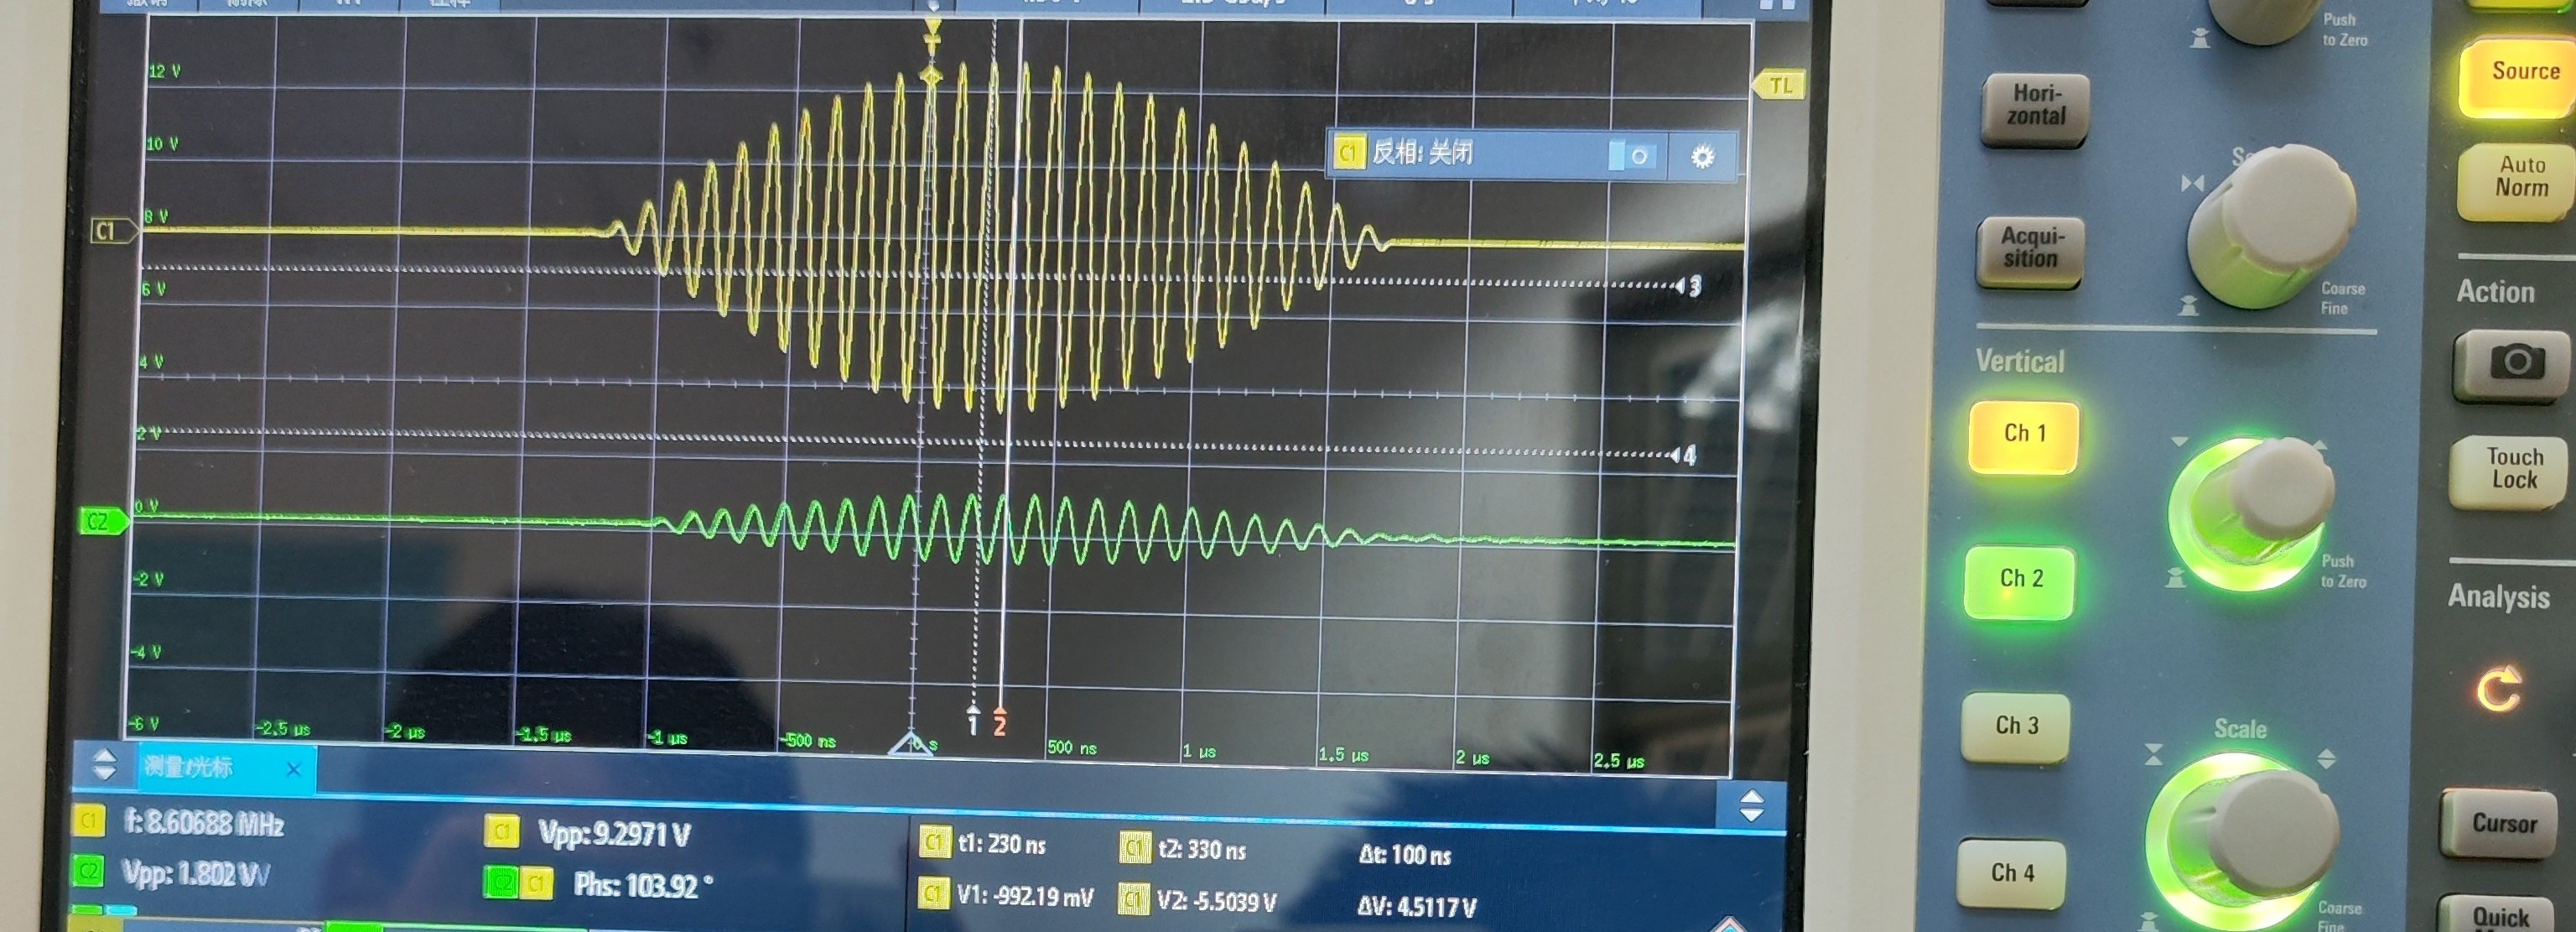
\includegraphics[width=\linewidth]{pic1.jpg}
	\caption{信号幅度最小的频率之一-$86kHz$}
	\label{fig:a5}
\end{figure}
\begin{figure}[htbp]
	\centering
	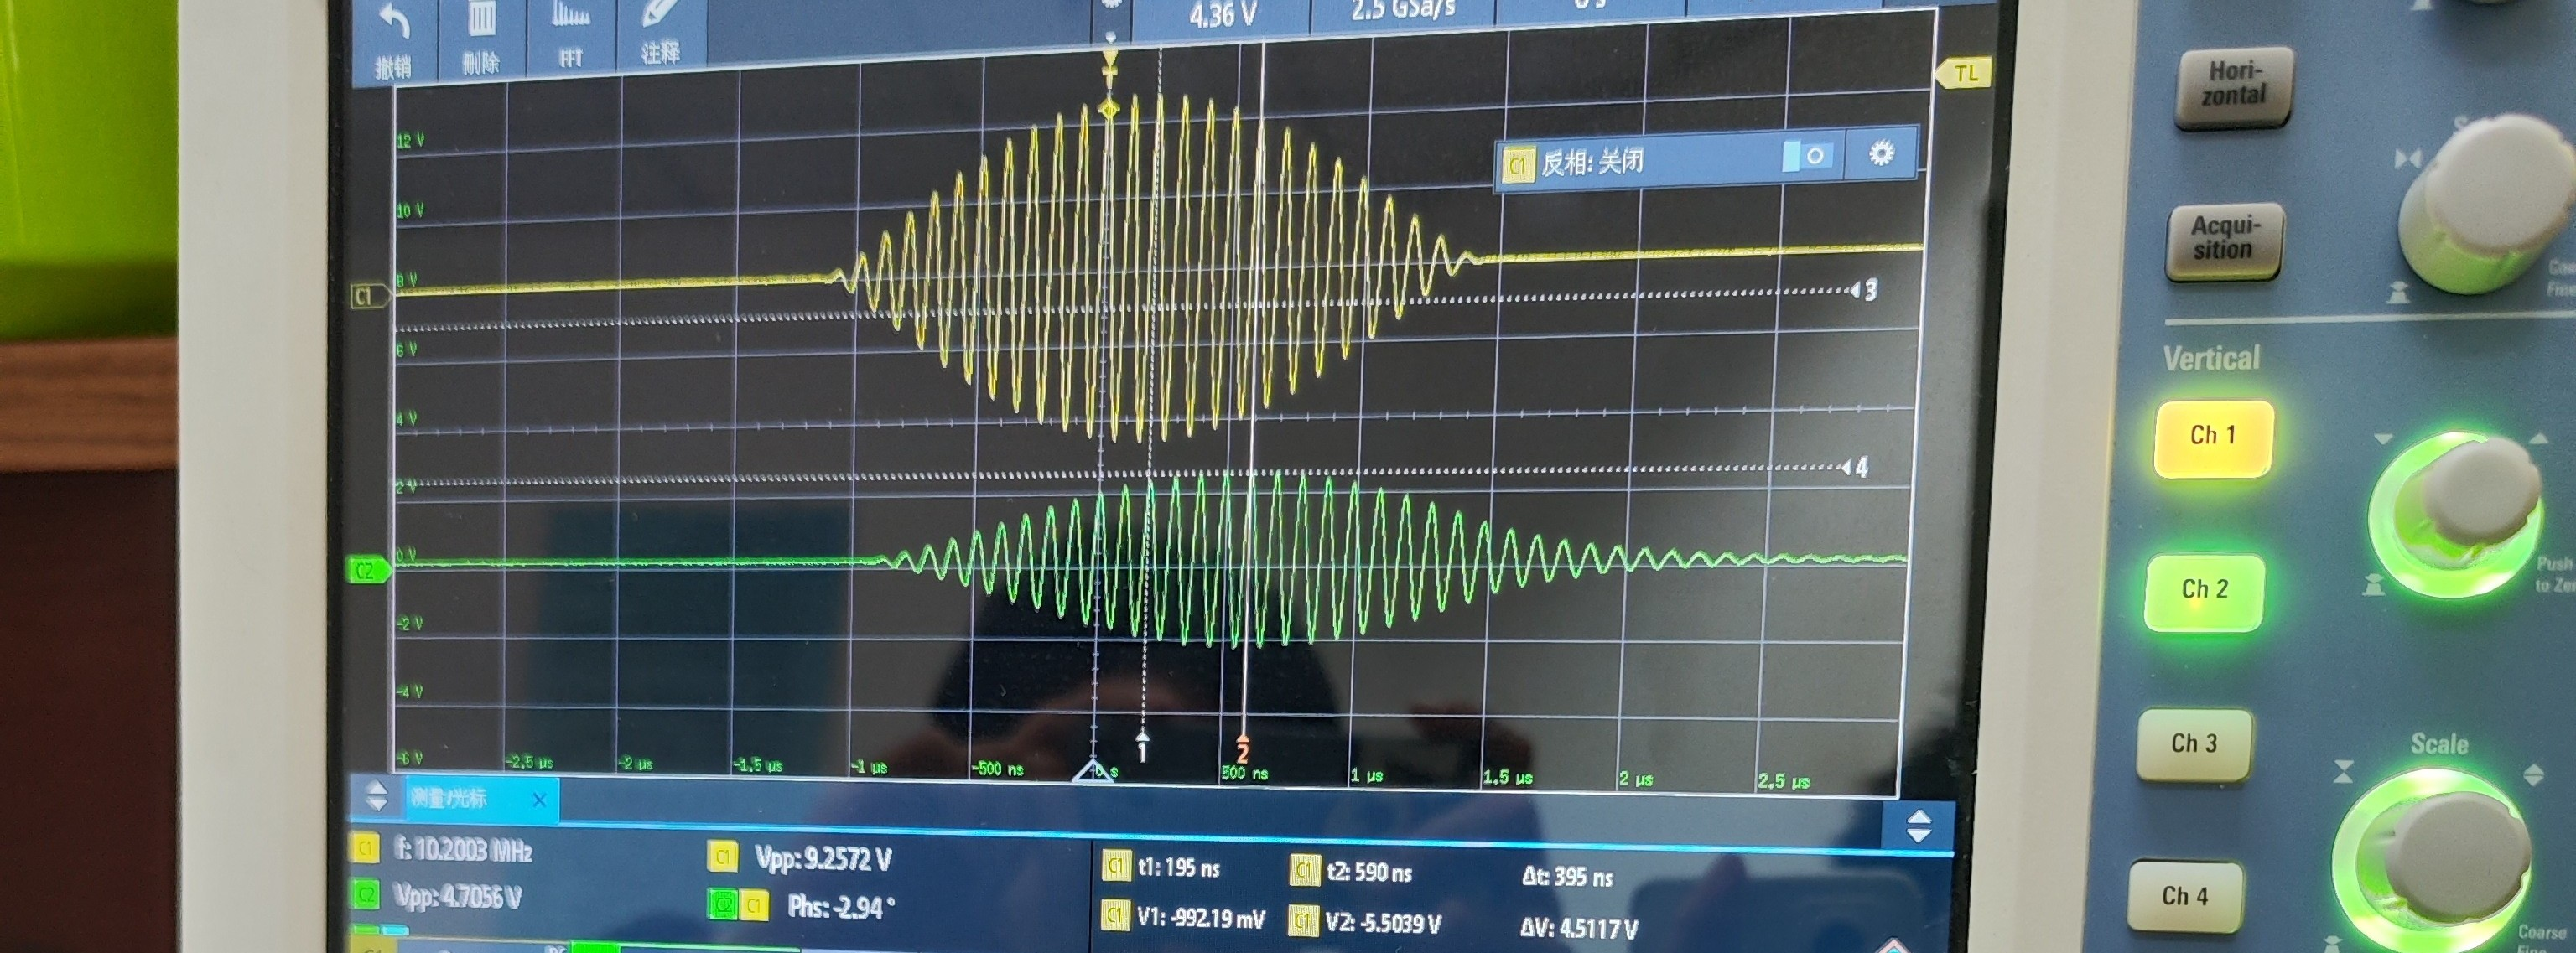
\includegraphics[width=\linewidth]{pic2.jpg}
	\caption{信号幅度最大且延时最长的1个频率-$102kHz$}
	\label{fig:a6}
\end{figure}
\begin{figure}[htbp]
	\centering
	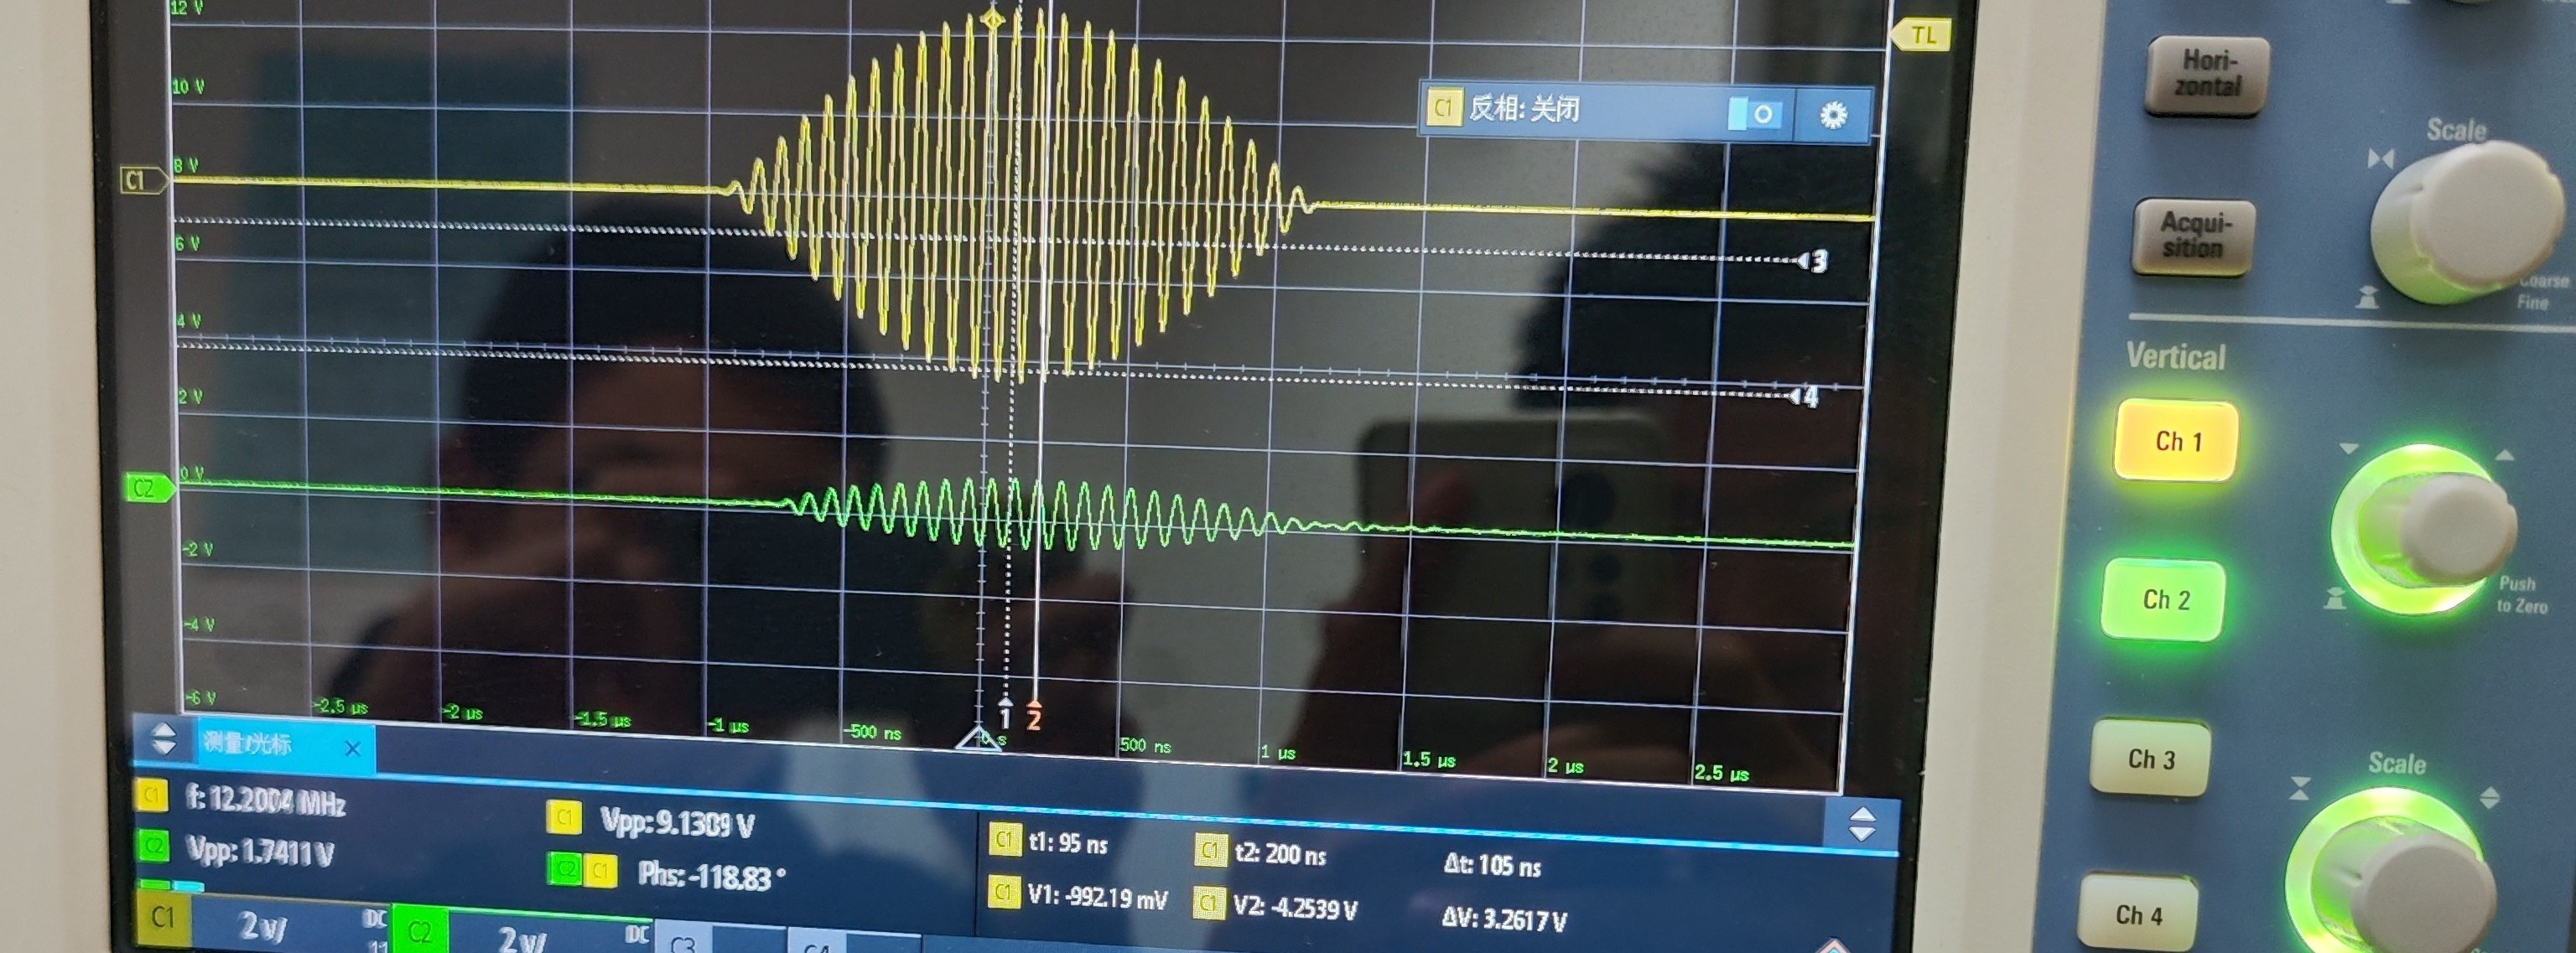
\includegraphics[width=\linewidth]{pic3.jpg}
	\caption{信号幅度最小的频率之一-$122kHz$}
	\label{fig:a7}
\end{figure}
\begin{figure}[htbp]
	\centering
	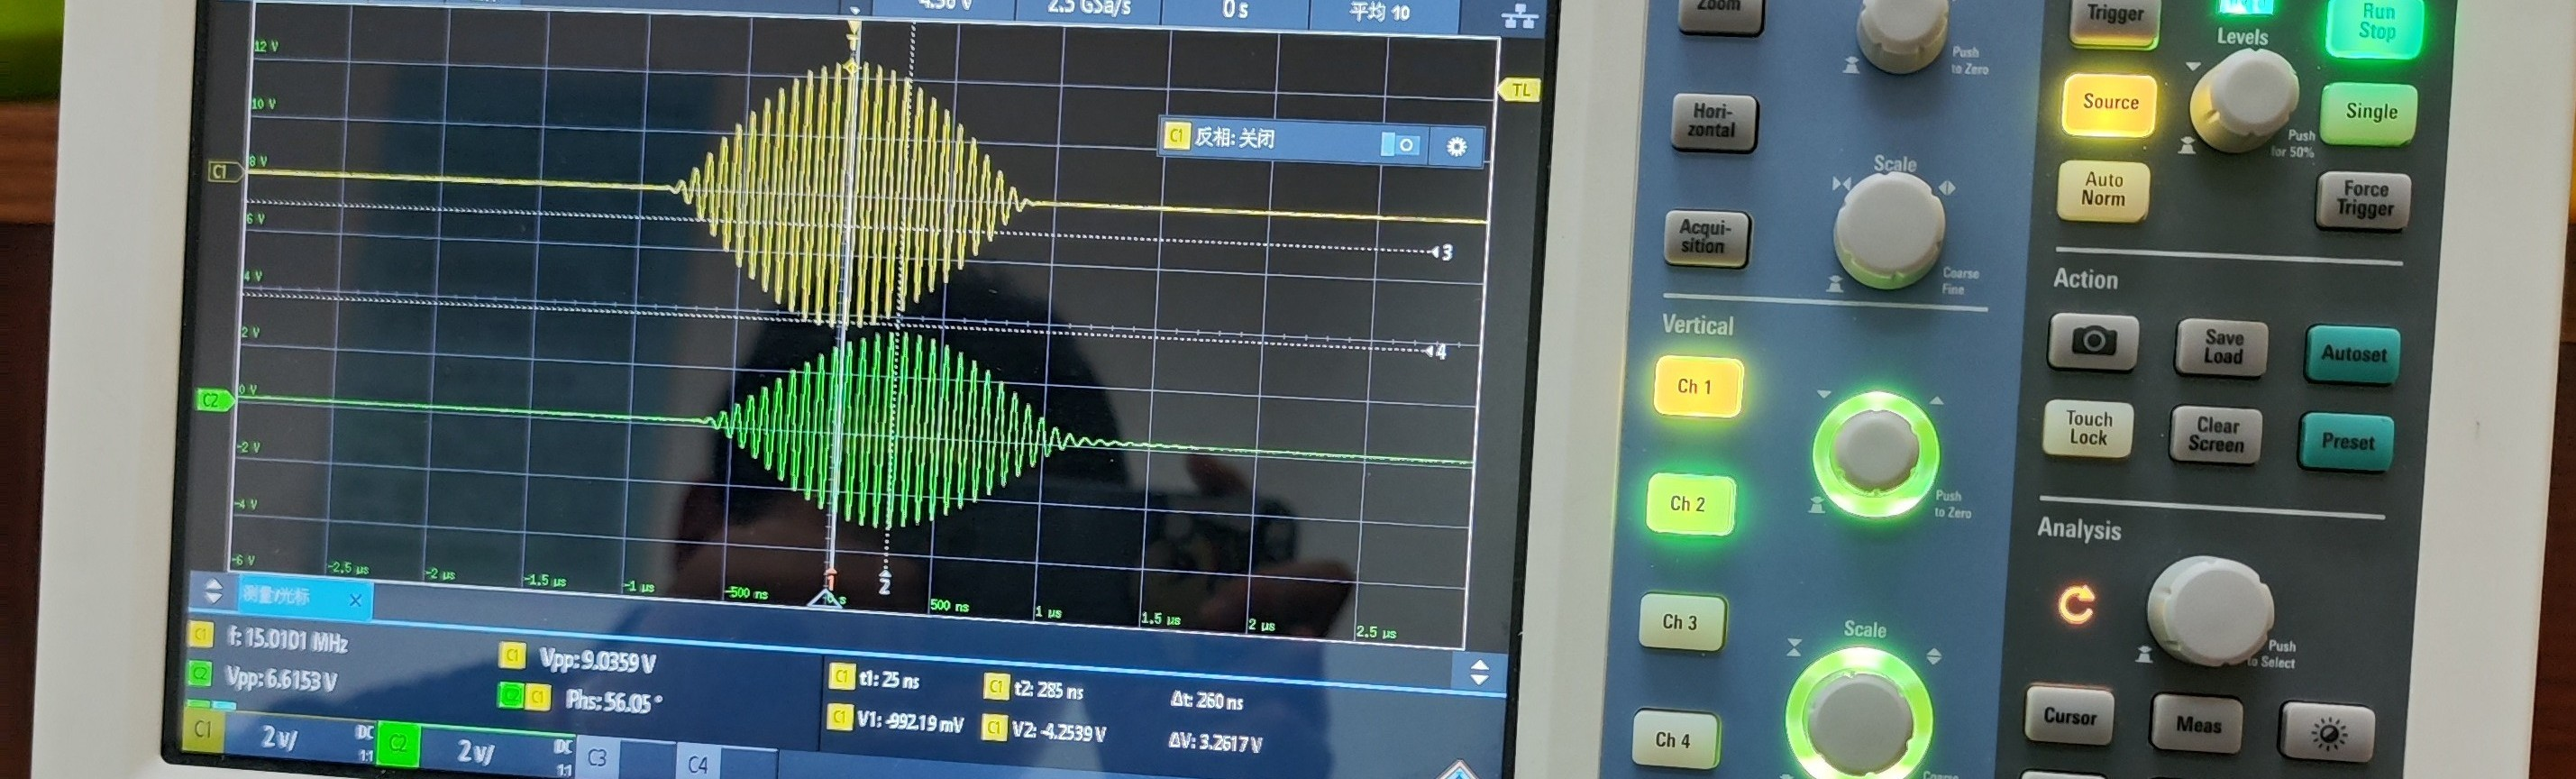
\includegraphics[width=\linewidth]{pic4.jpg}
	\caption{$150kHz$的波形}
	\label{fig:a8}
\end{figure}

现在进一步的计算这几种情况的群速度。我们用肉眼观察得到波包的“重心”,使用电缆总长$38.4m$除以重心的延时得到群速度。我们得到了:$86kHz$时,$v_g=3.84\times10^8m/s$;$102kHz$时,$v_g=9.72\times10^7m/s$,$122kHz$时,$v_g=3.66\times10^8m/s$,$150kHz$时,$v_g=1.48\times10^8m/s$。考虑到由目测读数带来的实验误差,我们可以近似认为所有情况都没有超光速,这是由于这里的波包携带了信息,信息的传递不能超光速。并且,我们看到对称性破缺带来的低速度仍然存在,与前面结果相符。

%------------------------------------------------

\section{同轴光子晶体的传输特性和群速度的理论预测}

同轴电缆电压和电流的通解是:$v=V_0^+e^{-\gamma x}+V_0^-e^{\gamma x}$,$i=\frac{1}{Z_0}(V_0^+e^{-\gamma x}-V_0^-e^{\gamma x})$,有待定参数$V_0^+$与$V_0^-$。我们加上已经知道同轴电缆的末端电压$v_2$与末端电流$i_2$,带入可得参数:$V_0^+=\frac{e^{\gamma l}v_2+Z_{01}e^{\gamma l}i_2}{2}$,$V_0^-=\frac{e^{-\gamma l}v_2-Z_{01}e^{-\gamma l}i_2}{2}$,这样一来,带入通解,就得到了始端电流电压,如下式:
\begin{equation*}
	\begin{bmatrix}
		v_1 \\
		i_1
	\end{bmatrix}=
	\begin{bmatrix}
		\cosh{\gamma l} & Z_{01}\sinh{\gamma l} \\
		\frac{1}{Z_{01}}\sinh{\gamma l} & \cosh{\gamma l}
	\end{bmatrix}
	\begin{bmatrix}
		v_2 \\
		i_2
	\end{bmatrix}
\end{equation*}
中间的这个矩阵就是传递矩阵。

针对我们的实验,我们需要考虑两段级联电缆,假设这两段电缆的传递矩阵分别为$A_1$,$A_2$,记$\begin{bmatrix}v_k\\i_k\end{bmatrix}=\vec{\xi_k}$,则:$\vec{\xi_1}=A_1\vec{\xi_2}=A_1A_2\vec{\xi_3}$,即整体的传递矩阵是$A_1A_2$。由该步骤,我们有了求解下面的思路:给几段电缆的传递矩阵相乘,就可以得到一个总的传递矩阵$A_T$。接下来,列出总的电路方程,设电源电动势为$e$,末端电流为$i_L$,并有负载电压$v_L$,最后可导出:$v_L=\frac{e}{[1\quad Z_0]A_T[1\quad 1/Z_0]^T}$,注意,这里得到的$v_L$为复数,按照前面的方法,就可以得到折射率,群速度的估计值了。对于传输效率,我们计算出最大输出功率以及模拟的功率,相除即可

用python编程,进行数值计算。模拟结果如图\ref{fig:a9},\ref{fig:a10},\ref{fig:a11},\ref{fig:a12}。
\begin{figure}[htbp]
	\centering
	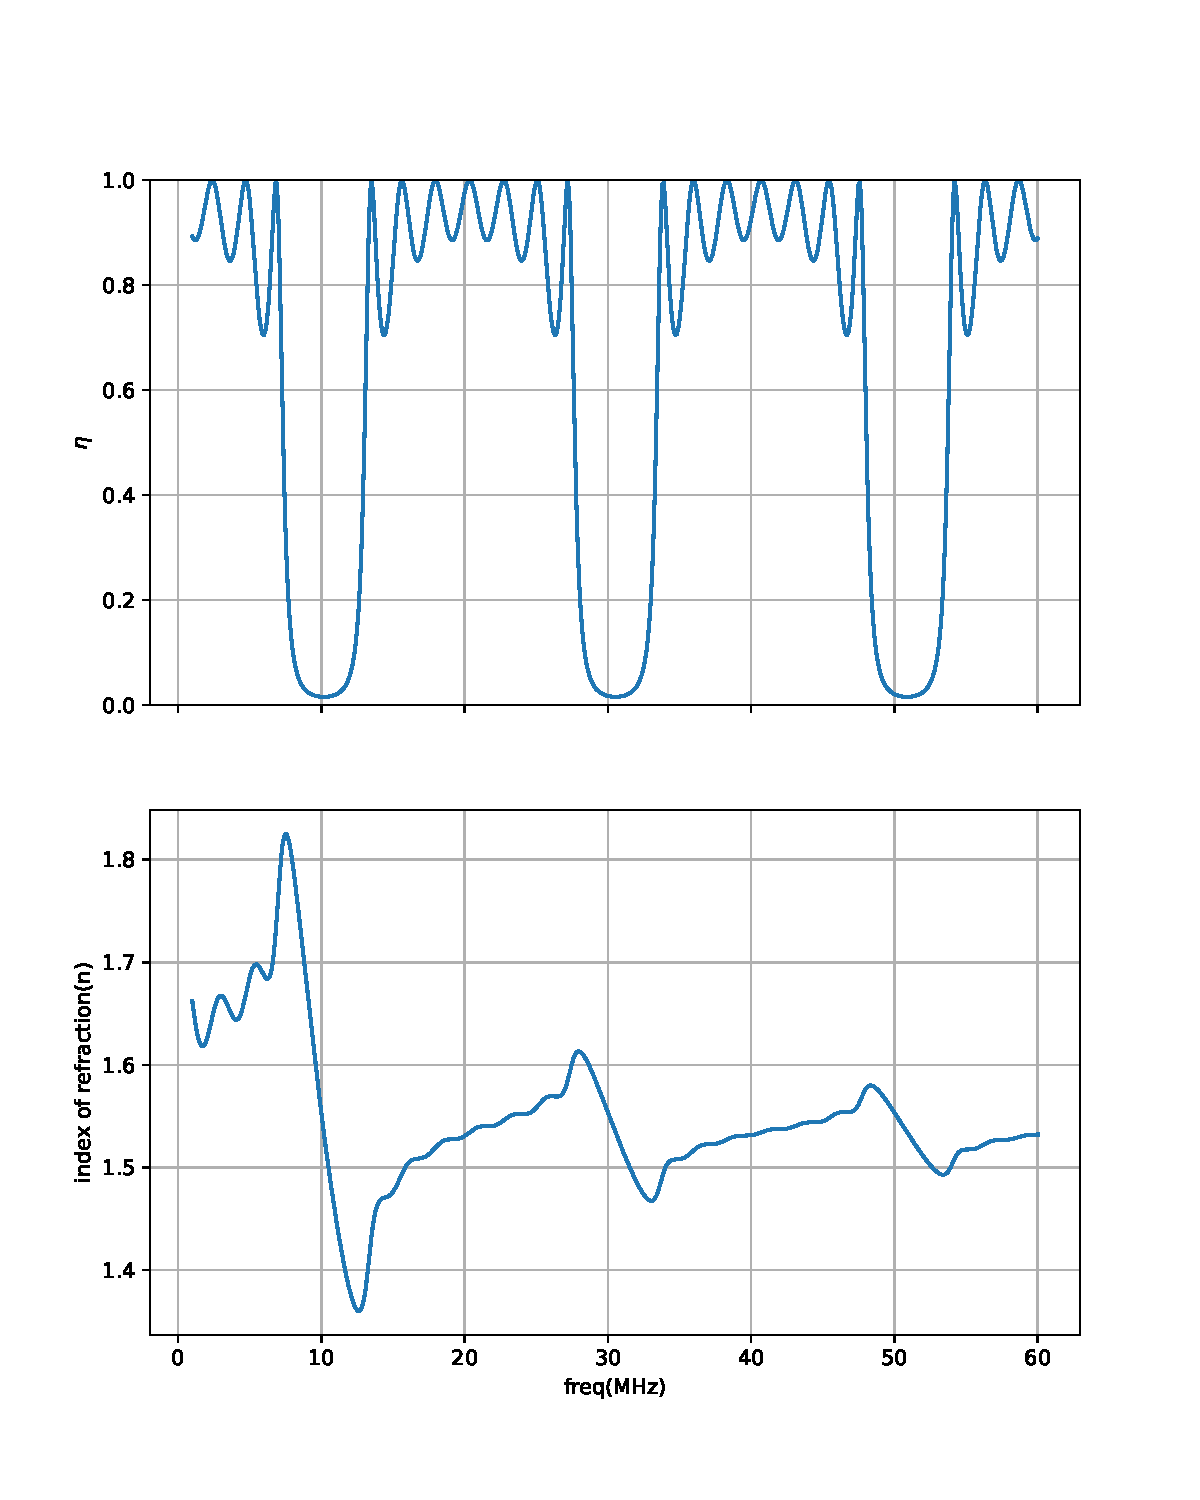
\includegraphics[width=\linewidth]{sim-eta-n.pdf}
	\caption{无缺陷的模拟传输效率和等效折射率}
	\label{fig:a9}
\end{figure}
\begin{figure}[htbp]
	\centering
	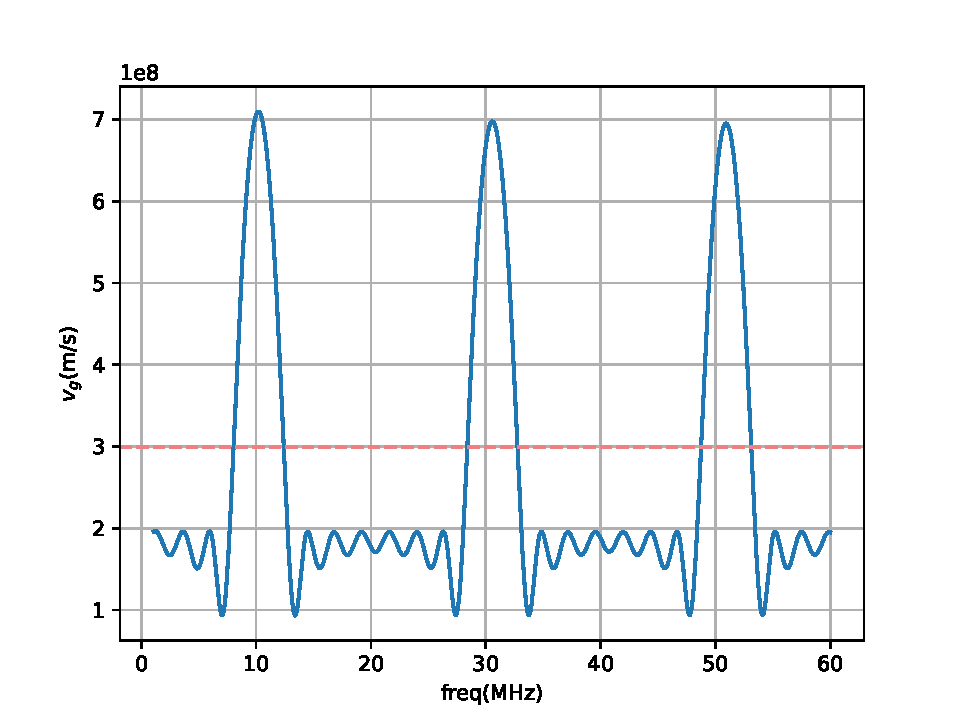
\includegraphics[width=\linewidth]{sim-vg.pdf}
	\caption{无缺陷的模拟群速度}
	\label{fig:a10}
\end{figure}
\begin{figure}[htbp]
	\centering
	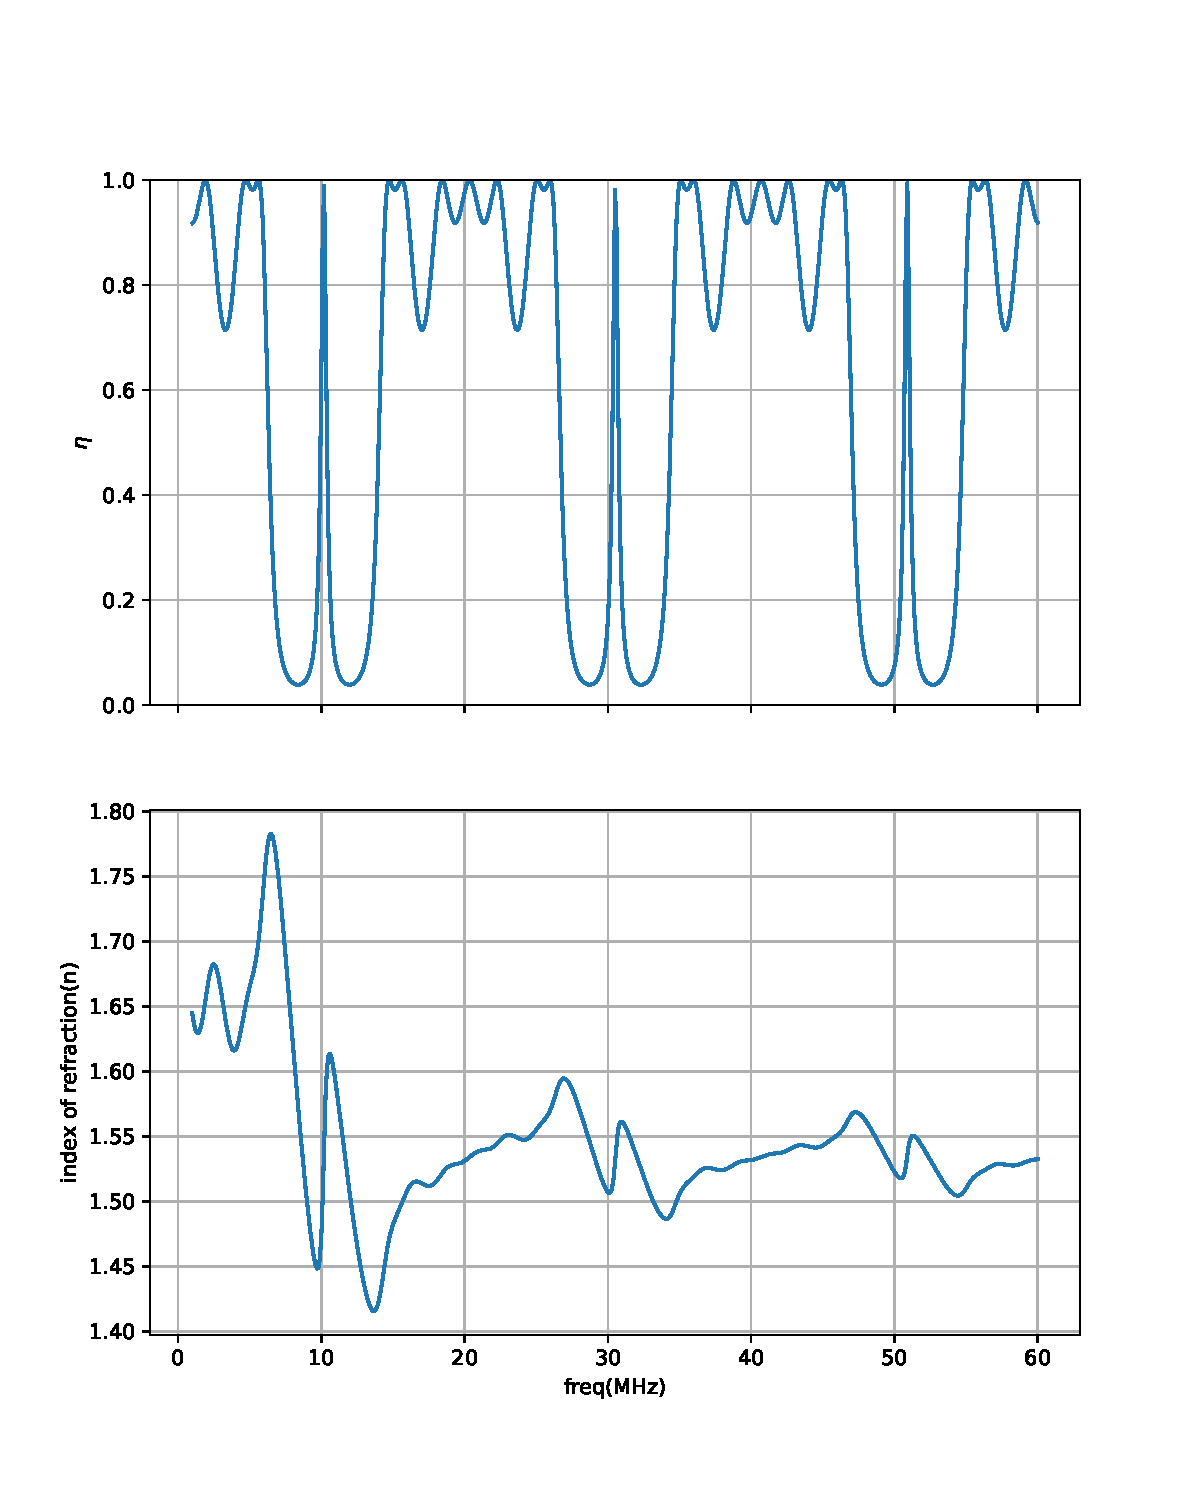
\includegraphics[width=\linewidth]{simd-eta-n.pdf}
	\caption{有缺陷的模拟传输效率和等效折射率}
	\label{fig:a11}
\end{figure}
\begin{figure}[htbp]
	\centering
	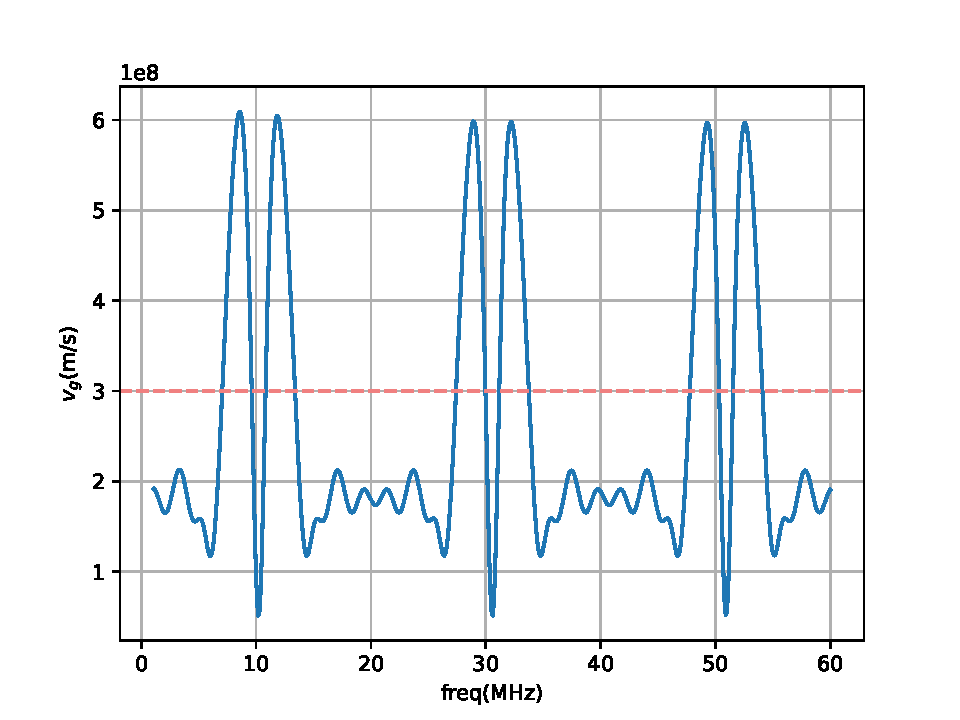
\includegraphics[width=\linewidth]{simd-vg.pdf}
	\caption{有缺陷的模拟群速度}
	\label{fig:a12}
\end{figure}

取出前$20MHz$的数据,与我们的测量值画在同一张图中,如图\ref{fig:a13},\ref{fig:a14},\ref{fig:a15},\ref{fig:a16}。可见我们的测量值十分贴合模拟值,测量的精度较高。另外,传输效率在低频时与模拟偏移过大,这值得仔细研究。
\begin{figure}[htbp]
	\centering
	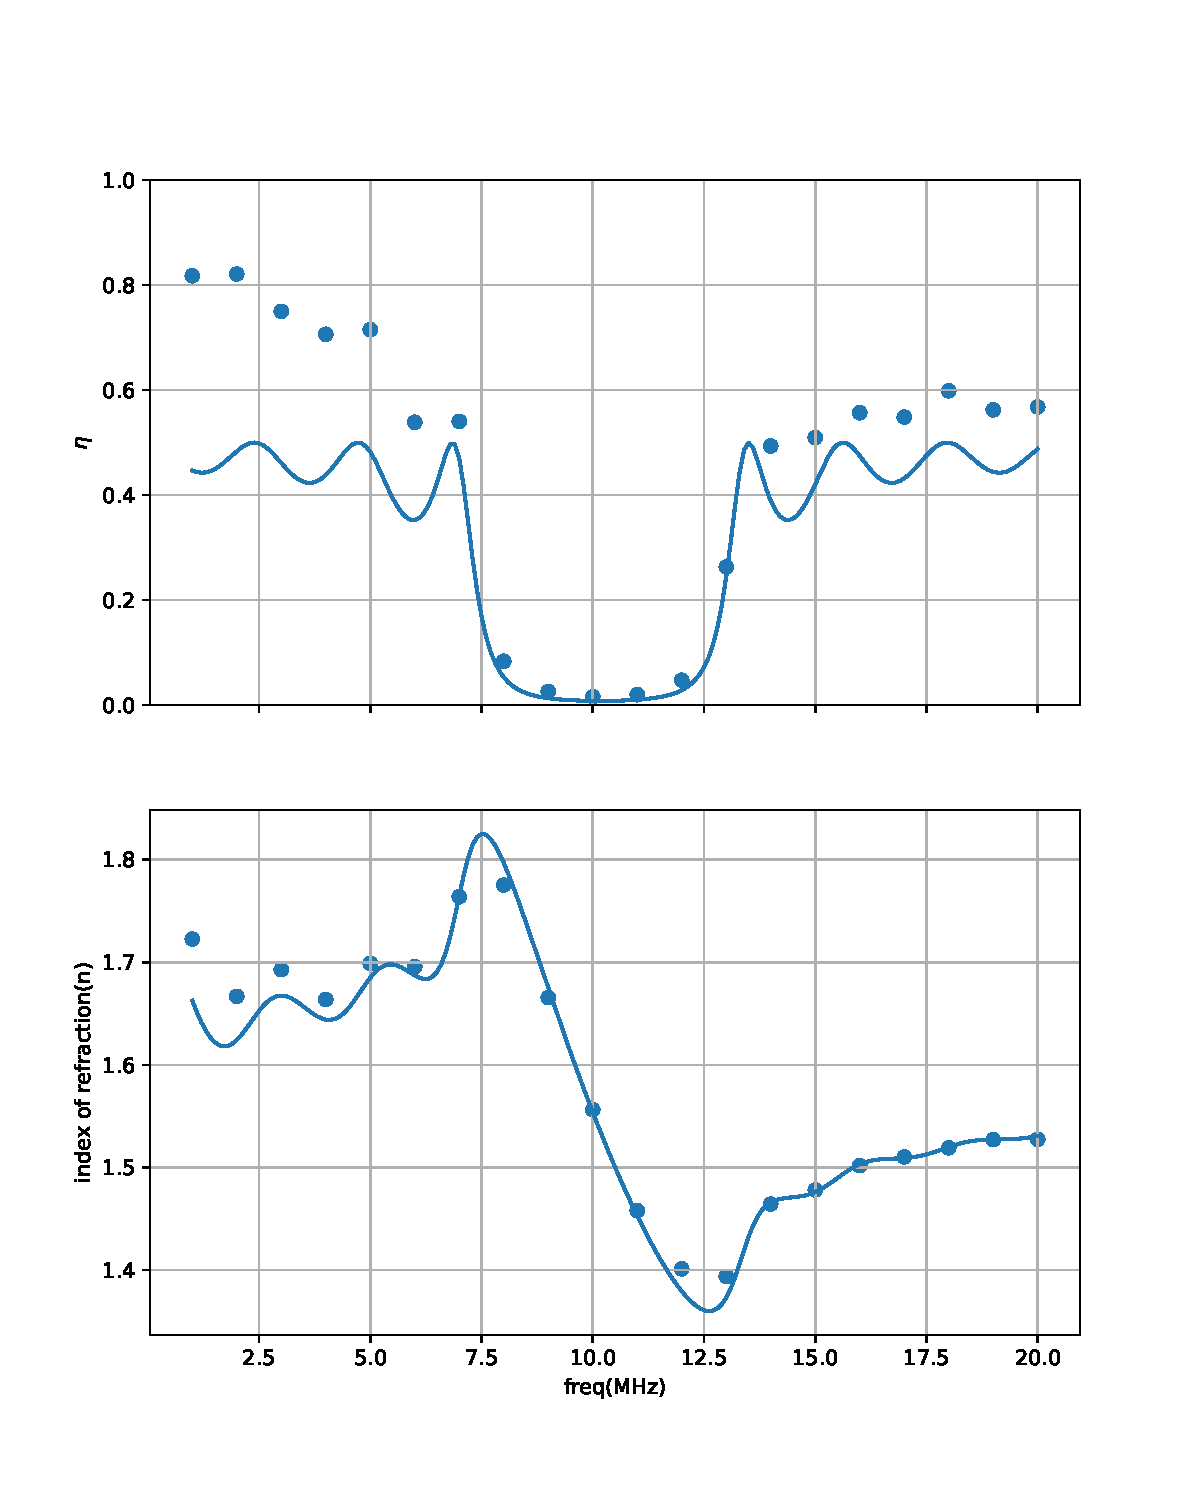
\includegraphics[width=\linewidth]{normal-eta-n.pdf}
	\caption{无缺陷的传输效率和等效折射率}
	\label{fig:a13}
\end{figure}
\begin{figure}[htbp]
	\centering
	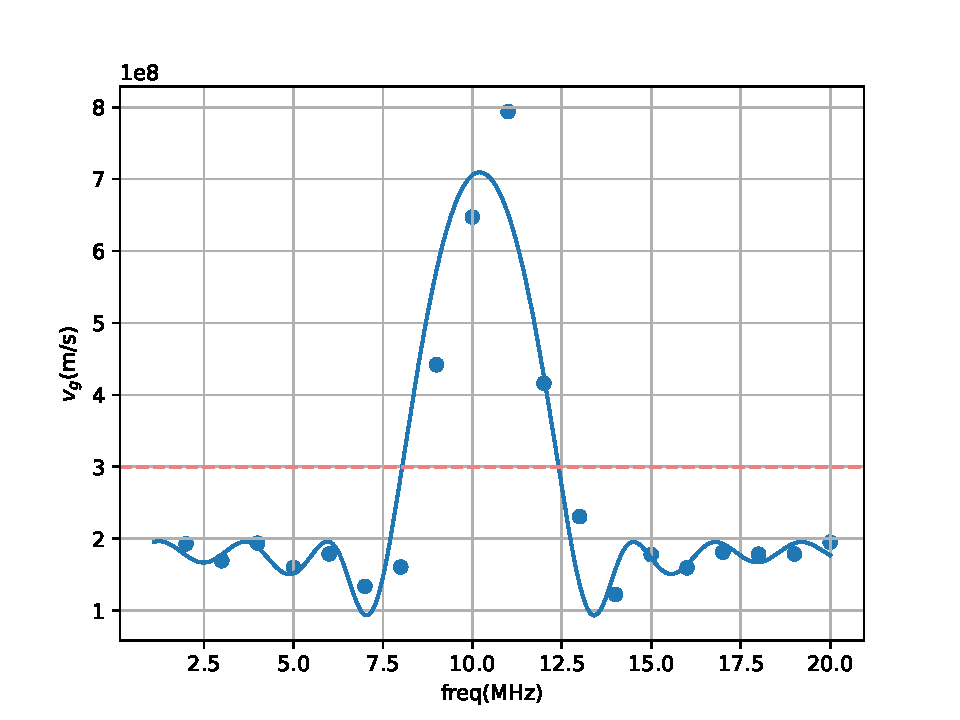
\includegraphics[width=\linewidth]{normal-vg.pdf}
	\caption{无缺陷的群速度}
	\label{fig:a14}
\end{figure}
\begin{figure}[htbp]
	\centering
	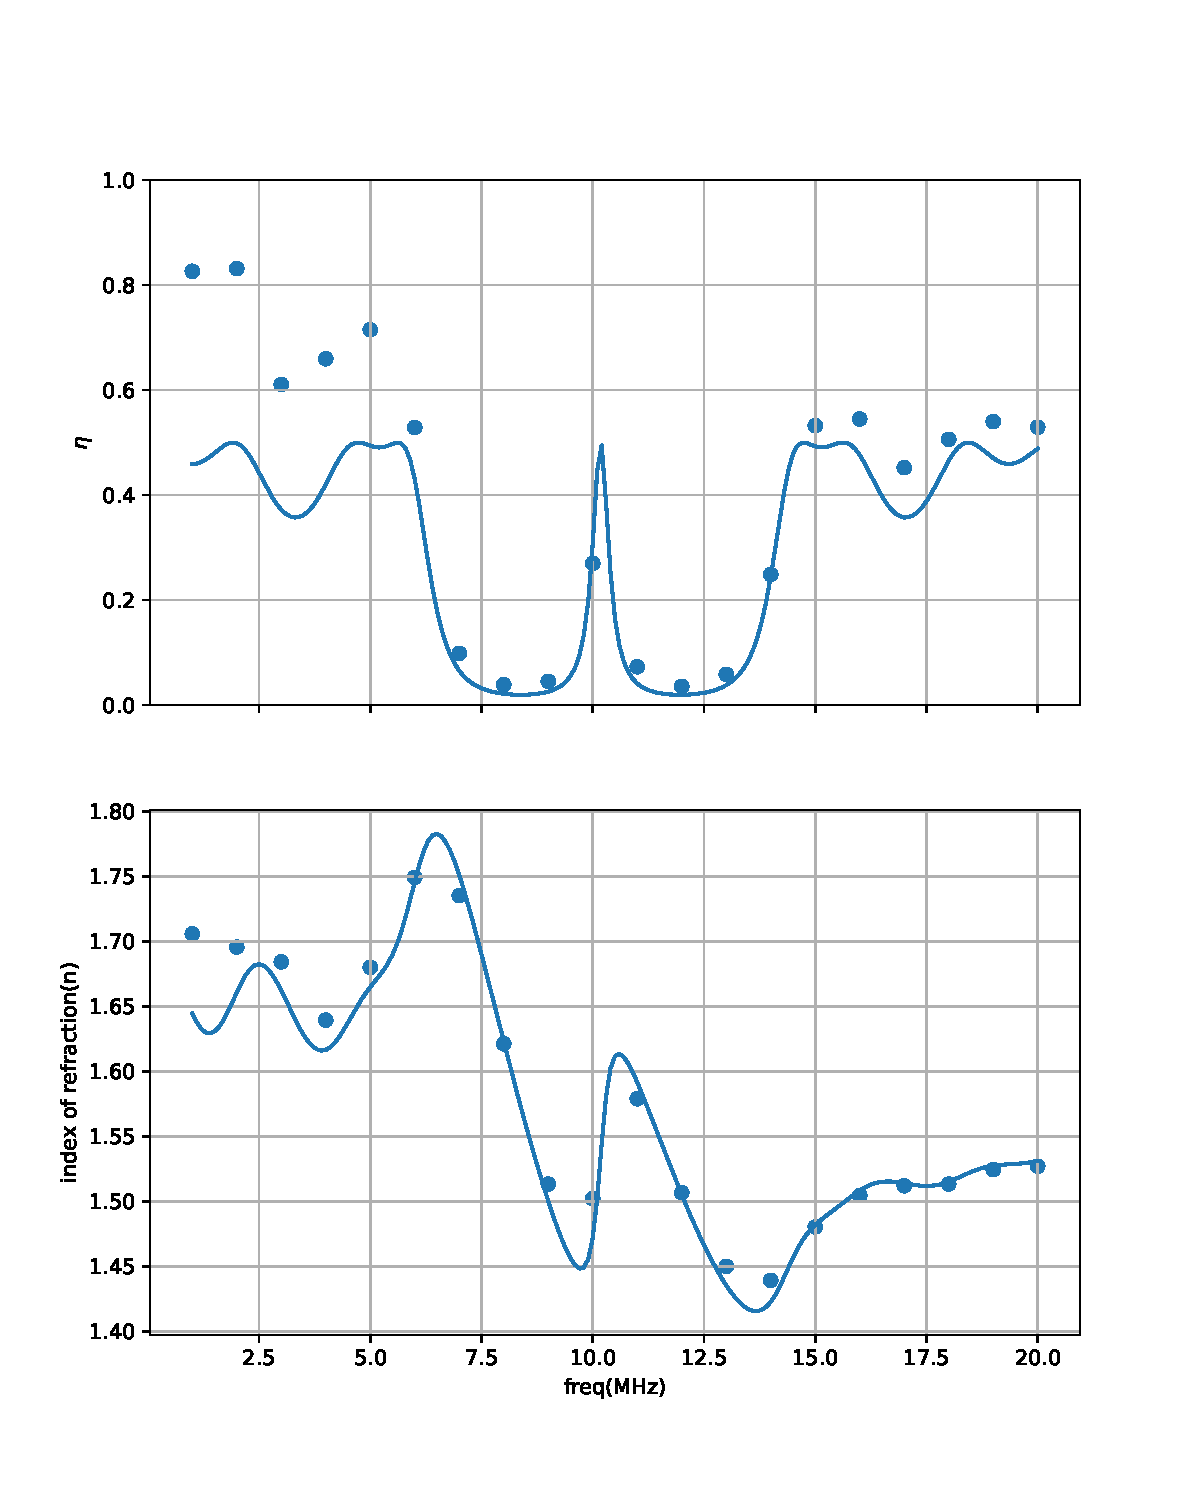
\includegraphics[width=\linewidth]{defects-eta-n.pdf}
	\caption{有缺陷的传输效率和等效折射率}
	\label{fig:a15}
\end{figure}
\begin{figure}[htbp]
	\centering
	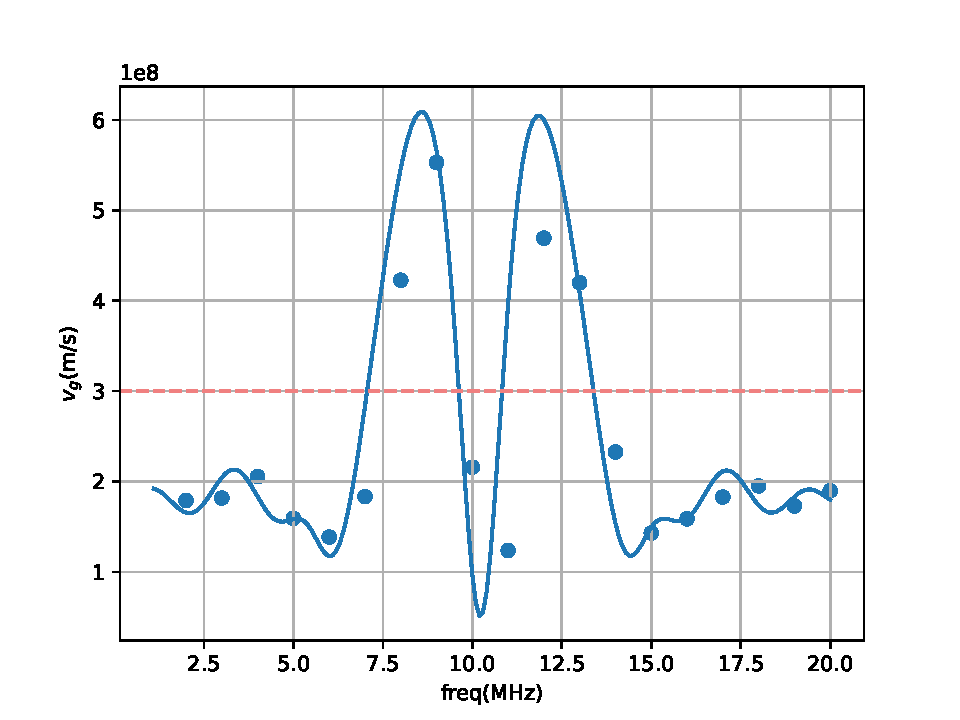
\includegraphics[width=\linewidth]{defects-vg.pdf}
	\caption{有缺陷的群速度}
	\label{fig:a16}
\end{figure}

%------------------------------------------------


%----------------------------------------------------------------------------------------
%	APPENDIX
%----------------------------------------------------------------------------------------

\clearpage
\appendix
\section{附录}
\renewcommand{\thetable}{附表\arabic{table}}
\setcounter{table}{0}

\begin{table}[h]
	\centering
	\begin{tabular}{|l|l|l|}
	\hline
	ch1(V) & ch2(V) & dphi    \\ \hline
	10.33  & 9.34   & -69.5   \\ \hline
	10.32  & 9.35   & -134.5  \\ \hline
	10.29  & 8.91   & 155.1   \\ \hline
	10.27  & 8.63   & 91.5    \\ \hline
	10.23  & 8.65   & 17.28   \\ \hline
	10.22  & 7.50   & -50.5   \\ \hline
	10.23  & 7.52   & -138.15 \\ \hline
	10.22  & 2.95   & 147.0   \\ \hline
	10.17  & 1.63   & 115.2   \\ \hline
	10.13  & 1.27   & 92.1    \\ \hline
	10.15  & 1.42   & 72.9    \\ \hline
	10.12  & 2.20   & 41.54   \\ \hline
	10.10  & 5.18   & -11.19  \\ \hline
	10.08  & 7.08   & -107.19 \\ \hline
	10.06  & 7.18   & -174.61 \\ \hline
	10.32  & 7.70   & 110.50  \\ \hline
	10.02  & 7.42   & 44.08   \\ \hline
	9.98   & 7.72   & -23.31  \\ \hline
	9.95   & 7.46   & -90.69  \\ \hline
	9.94   & 7.49   & -152.64 \\ \hline
	\end{tabular}
	\caption{无缺陷时的测定数据}
	\label{tab:app1}
\end{table}

\begin{table}[h]
	\centering
	\begin{tabular}{|c|c|c|}
	\hline
	频率(MHz) & $\eta$ & n     \\ \hline
	1       & 0.818  & 1.723 \\ \hline
	2       & 0.821  & 1.667 \\ \hline
	3       & 0.75   & 1.693 \\ \hline
	4       & 0.706  & 1.664 \\ \hline
	5       & 0.715  & 1.699 \\ \hline
	6       & 0.539  & 1.696 \\ \hline
	7       & 0.54   & 1.764 \\ \hline
	8       & 0.083  & 1.775 \\ \hline
	9       & 0.026  & 1.666 \\ \hline
	10      & 0.016  & 1.556 \\ \hline
	11      & 0.02   & 1.458 \\ \hline
	12      & 0.047  & 1.401 \\ \hline
	13      & 0.263  & 1.394 \\ \hline
	14      & 0.493  & 1.464 \\ \hline
	15      & 0.509  & 1.478 \\ \hline
	16      & 0.557  & 1.502 \\ \hline
	17      & 0.548  & 1.51  \\ \hline
	18      & 0.598  & 1.519 \\ \hline
	19      & 0.562  & 1.527 \\ \hline
	20      & 0.568  & 1.528 \\ \hline
	\end{tabular}
	\caption{无缺陷时的传输效率和等效折射率}
	\label{tab:app2}
\end{table}

\begin{table}[h]
	\centering
	\begin{tabular}{|c|c|}
	\hline
	频率(MHz) & $v_g$($1\times10^8$m/s)    \\ \hline
	2    & 1.928 \\ \hline
	3    & 1.693 \\ \hline
	4    & 1.938 \\ \hline
	5    & 1.599 \\ \hline
	6    & 1.788 \\ \hline
	7    & 1.338 \\ \hline
	8    & 1.606 \\ \hline
	9    & 4.419 \\ \hline
	10   & 6.472 \\ \hline
	11   & 7.938 \\ \hline
	12   & 4.161 \\ \hline
	13   & 2.307 \\ \hline
	14   & 1.224 \\ \hline
	15   & 1.779 \\ \hline
	16   & 1.595 \\ \hline
	17   & 1.812 \\ \hline
	18   & 1.785 \\ \hline
	19   & 1.787 \\ \hline
	20   & 1.952 \\ \hline
	\end{tabular}
	\caption{无缺陷时的群速度}
	\label{tab:app3}
\end{table}

\begin{table}[h]
	\centering
	\begin{tabular}{|c|c|c|}
	\hline
	ch1(V)& ch2(V)  & dphi    \\ \hline
	10.32 & 9.38 & -78.66  \\ \hline
	10.31 & 9.40 & -156.38 \\ \hline
	10.29 & 8.04 & 127.0   \\ \hline
	10.27 & 8.34 & 57.6    \\ \hline
	10.22 & 8.64 & -27.36  \\ \hline
	10.22 & 7.43 & -124.0  \\ \hline
	10.23 & 3.21 & 159.89  \\ \hline
	10.21 & 2.01 & 121.92  \\ \hline
	10.17 & 2.16 & 91.94   \\ \hline
	10.13 & 5.26 & 27.36   \\ \hline
	10.16 & 2.74 & -80.88  \\ \hline
	10.15 & 1.91 & -113.68 \\ \hline
	10.13 & 2.45 & -149.22 \\ \hline
	10.11 & 5.04 & 150.84  \\ \hline
	10.09 & 7.36 & 56.05   \\ \hline
	10.08 & 7.44 & -30.00  \\ \hline
	10.04 & 6.75 & -105.31 \\ \hline
	10.01 & 7.12 & -176.12 \\ \hline
	9.99  & 7.34 & 104.43  \\ \hline
	9.98  & 7.26 & 31.68   \\ \hline
	\end{tabular}
	\caption{有缺陷时的测定数据}
	\label{tab:app4}
\end{table}

\begin{table}[h]
	\centering
	\begin{tabular}{|c|c|c|}
	\hline
	频率(MHz) & $\eta$ & n     \\ \hline
	1      & 0.826  & 1.706 \\ \hline
	2      & 0.831  & 1.696 \\ \hline
	3      & 0.61   & 1.684 \\ \hline
	4      & 0.659  & 1.639 \\ \hline
	5      & 0.715  & 1.68  \\ \hline
	6      & 0.529  & 1.749 \\ \hline
	7      & 0.098  & 1.735 \\ \hline
	8      & 0.039  & 1.621 \\ \hline
	9      & 0.045  & 1.513 \\ \hline
	10     & 0.27   & 1.502 \\ \hline
	11     & 0.073  & 1.579 \\ \hline
	12     & 0.035  & 1.507 \\ \hline
	13     & 0.058  & 1.45  \\ \hline
	14     & 0.249  & 1.439 \\ \hline
	15     & 0.532  & 1.48  \\ \hline
	16     & 0.545  & 1.504 \\ \hline
	17     & 0.452  & 1.512 \\ \hline
	18     & 0.506  & 1.513 \\ \hline
	19     & 0.54   & 1.524 \\ \hline
	20     & 0.529  & 1.527 \\ \hline
	\end{tabular}
	\caption{有缺陷时的传输效率和等效折射率}
	\label{tab:app5}
\end{table}

\begin{table}[h]
	\centering
	\begin{tabular}{|c|c|}
	\hline
	频率$MHz$ & $v_g$($1\times10^8$m/s) \\ \hline
	2       & 1.79                    \\ \hline
	3       & 1.817                   \\ \hline
	4       & 2.053                   \\ \hline
	5       & 1.592                   \\ \hline
	6       & 1.385                   \\ \hline
	7       & 1.832                   \\ \hline
	8       & 4.226                   \\ \hline
	9       & 5.529                   \\ \hline
	10      & 2.158                   \\ \hline
	11      & 1.237                   \\ \hline
	12      & 4.691                   \\ \hline
	13      & 4.198                   \\ \hline
	14      & 2.325                   \\ \hline
	15      & 1.43                    \\ \hline
	16      & 1.586                   \\ \hline
	17      & 1.827                   \\ \hline
	18      & 1.951                   \\ \hline
	19      & 1.729                   \\ \hline
	20      & 1.897                   \\ \hline
	\end{tabular}
	\caption{有缺陷时的群速度}
	\label{tab:app6}
\end{table}

%----------------------------------------------------------------------------------------

\end{document}
